Es werden zwei Messungen durchgeführt und ausgewertet. Das Ziel der Messungen ist es, die Lichtgeschwindigkeit bestimmen zu können. Es wird die Verschiebung der Position des Lichtbündels $x$ in Funktion der Drehfrequenz $f$ ausgemessen. \\
\\
An die Messdaten wird dann folgende Fitfunktion, welche aus der Formel \ref{eq:Formel_Lichtgeschwindigkeit_Michelson} abgeleitet wurde, angelegt:\\

%%%%%%%%%%%%%%%%%%%%%%%%%%%%%%%%%%%%%%%%%%%%%%%%%%%%%%%%%%%%%%%%%%%%%%%%%%%%%
\begin{equation}
x = 4\cdot 2 \cdot f \cdot \dfrac{f_{1} \cdot (s_{2}+f_{2})}{c}
\label{eq:Formel_Lichtgeschwindigkeit_Michelson_2}
\end{equation}
%%%%%%%%%%%%%%%%%%%%%%%%%%%%%%%%%%%%%%%%%%%%%%%%%%%%%%%%%%%%%%%%%%%%%%%%%%%%%

\begin{tabbing}
\hspace{10mm}			\=  \hspace{60mm} \=	\\
mit	\>					\\
$x$	\> Verschiebung des Lichbündels		\> 	[m]	\\
$f$	\> Frequenz des Drehspiegels		\>	[Hz]	\\
$c$	\> Lichtgeschwindigkeit			\> 	[m/s]	\\
\\
$f_1$	\> Distanz Linse-Spalt			\> 	1 m	\\
$f_2$	\> Distanz Hohlspiegel-Endspiegel	\> 	4.82 m \\
$s_2$	\> Distanz Hohlspiegel-Drehspiegel	\> 	4.75 m \\
\end{tabbing}

%%%%%%%%%%%%%%%%%%%%%%%%%%%%%%%%%%%%%%%%%%%%%%%%%%%%%%%%%%%%%%%%%%%%%%%%%%%%%
\begin{figure}[h]
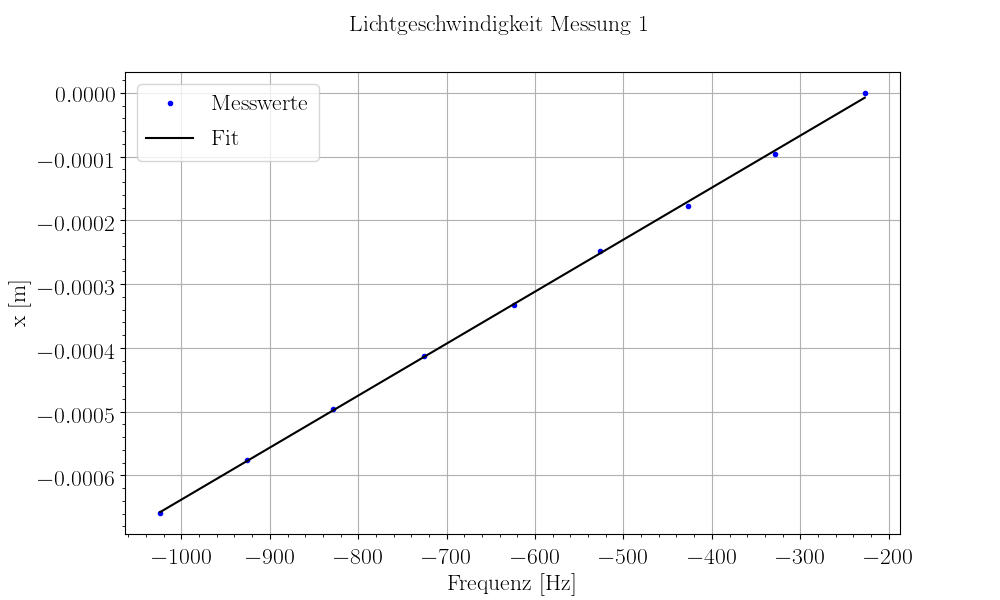
\includegraphics[width=\textwidth]{graphics/messung_1.png}
\caption{Lichtgeschwindigkeitsmessung aus dem Abstand der Lichtbündel bei verschiedenen Frequenzen eines Drehspiegels} % picture caption
\label{fig:pol1}
\end{figure}
%%%%%%%%%%%%%%%%%%%%%%%%%%%%%%%%%%%%%%%%%%%%%%%%%%%%%%%%%%%%%%%%%%%%%%%%%%%%%

\textbf{Resultat: $c = (294.84 \pm 2.16) \cdot 10^6 m/s$}\\
\\
Dieser Wert liegt bereits sehr nahe an der gewünschten Geschwindigkeit welche im Kapitel \ref{sec:Äussere Einflüsse} berechnet wurde. Um einen zweiten Vergleichswert zu erhalten, wurde die Messung ein zweites Mal durchgeführt. Dabei wurden die Rollen des Versuchleiters und Assistenten getauscht.
\clearpage

%%%%%%%%%%%%%%%%%%%%%%%%%%%%%%%%%%%%%%%%%%%%%%%%%%%%%%%%%%%%%%%%%%%%%%%%%%%%%
\begin{figure}[ht]
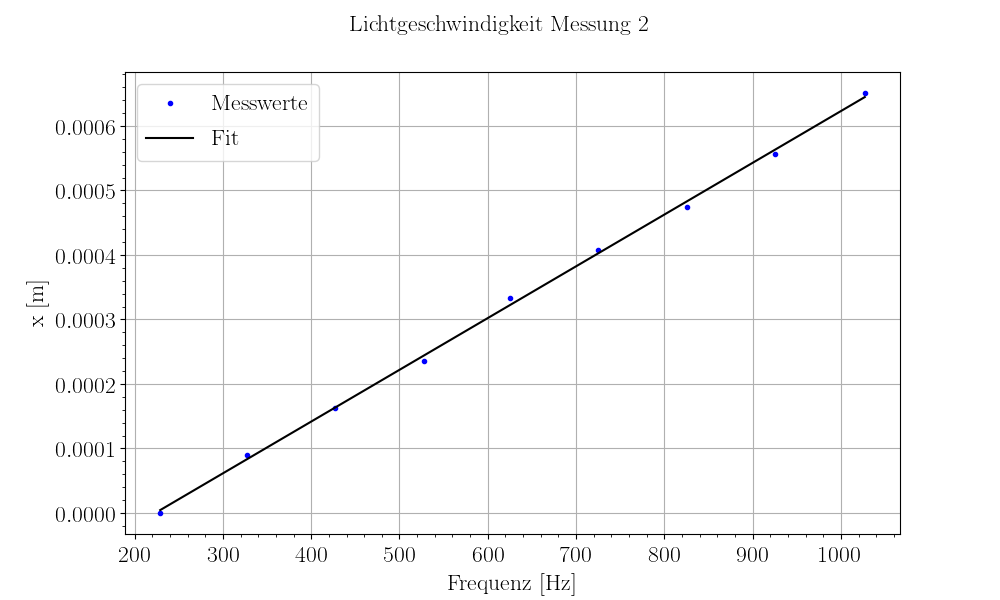
\includegraphics[width=\textwidth]{graphics/messung_2.png}
\caption{Lichtgeschwindigkeitsmessung aus dem Abstand der Lichtbündel bei verschiedenen Frequenzen eines Drehspiegels} % picture caption
\label{fig:pol1}
\end{figure}
%%%%%%%%%%%%%%%%%%%%%%%%%%%%%%%%%%%%%%%%%%%%%%%%%%%%%%%%%%%%%%%%%%%%%%%%%%%%%
\textbf{Resultat: $c = (299.84 \pm 3.83) \cdot 10^6 m/s$}\\
\\
Dieses Resultat liegt nun sehr nahe am gewünschten Wert. Die erhaltenen Daten müssen nun noch mittels Fehlerrechnung exakt berechnet werden und können dann im Kapitel Resultate miteinander verglichen werden.
